\chapter{Related Work}

\section{Habit Formation}

\subsection{Habit Formation and User Interface}
Previous work has been done to tie habit formation with online user interfaces \cite{johnson2013designing}. In this book, Dr. Jeff Johnson describes how psychology ties into user interface design. He cites that familiar user interfaces lead to less mental stress, encouraging users to come back to your application repeatedly since it seems familiar and less stressful to them. We desire users to consistently use our application every day, so we must keep this in mind.

\subsection{Memrise}
As mentioned before, Memrise is an excellent example of habit formation. In one paper, researchers gauged the ability of students to memorise simple Latin phrases in a classroom setting. They found that Memrise is an effective tool 

\subsection{Gamification}
Gamification in the classroom has several other examples that can be compared to our application.

\subsection{Classcraft}
Classcraft is an intriguing example of gamification in education (See \textbf{\hyperref[fig:classcraft]{Figure \ref*{fig:classcraft}}}). In Classcraft, students choose a "role" and go on the equivalent of a World of Warcraft raid with their fellow classmates. Classcraft is interesting in that it promotes co-operation and a variety of skills, so that students can assist each other where they might not have a certain skill. 

Classcraft takes the typical elements of an RPG and converts them into an experience that supplements a typical classroom experience.

\begin{figure}[h]
	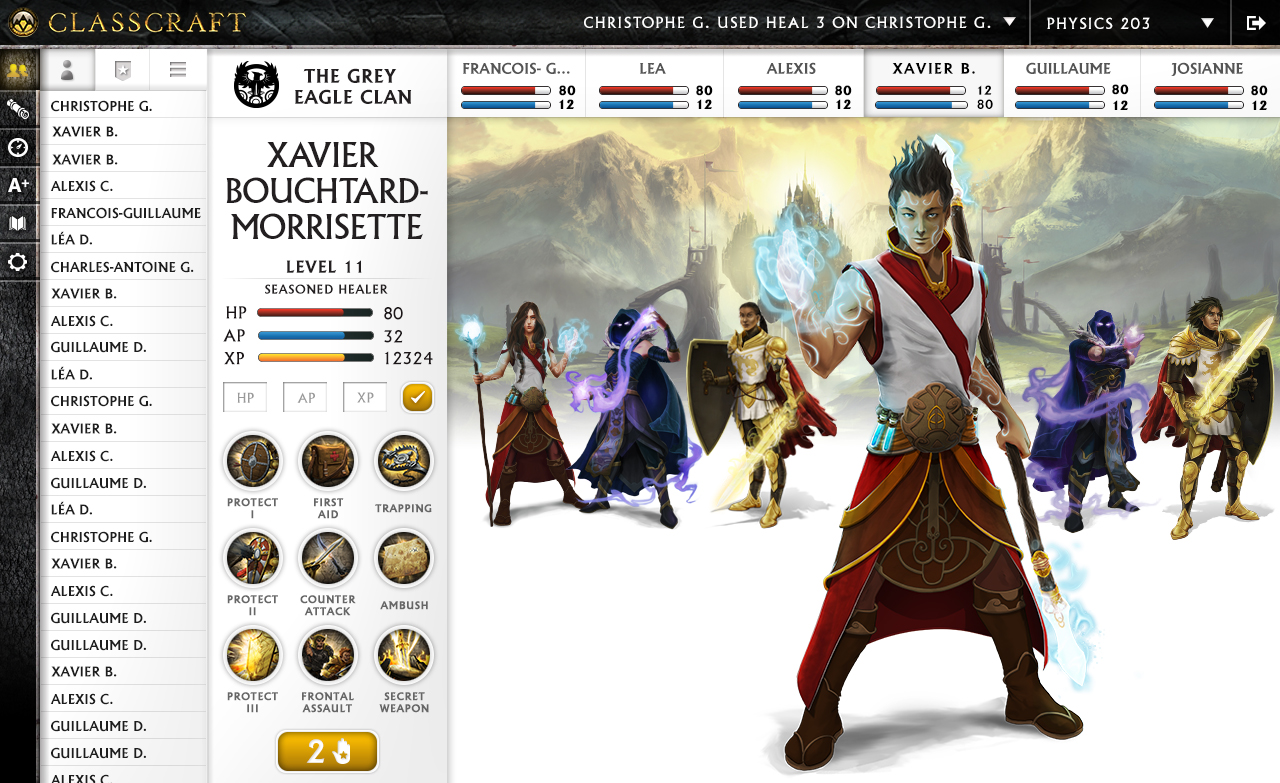
\includegraphics[width=1.0\linewidth]{figures/classcraft}
	\caption{Classcraft user interface. Note the student's health and mana pool, as well as the list of other students in the classroom.}
	\label{fig:classcraft}
	\cite{hardy_heyes_1999}
\end{figure}

Interesting to note is the emphasis Classcraft puts on integration with existing technologies such as Google Classroom. In order for this application to be widely adopted, it is definitely necessary to have the experience of the teacher go extremely smoothly. Thus, if an application ties directly in with existing technology that the teacher is already familiar with, it will be much more readily adopted by the educational community. It's important to value the teacher's time with this application, so it is necessary to make the UI recognizable, familiar and easy to work with, as well as integrating it with existing tools and perhaps even modeling the user interface after tools that many teachers will already be familiar with.